\chapter{Globally hyperbolic spacetime}\label{chapter:4}

\red{Numerare equazioni, aggiungiere riferimenti}\\
\red{nelle prime sezioni vanno aggiunte ancora cose}\\
\red{aggiungiere le def in $\A^{2,1}$ e dire che è uguale a farlo in $\AS^2,1$}\\
From now on we will only work with Lorentzian manifold of dimension $(2+1)$.

%Def di acausal set in \AS e \A (magari diretto come grafico)
%Lemma di caratt. degli acausal set come grafico
% Def di spacelike surface
% Spacelike surfaces sono acausal
%def di invisible domain 
%def di achronal meridian
\section{Achronal and acausal set}
\red{veloce intro, magari mettere alcuni risultati con o senza dim}

\begin{definition}
    A subset $X \subset \AS^{2,1} \cup \partial\AS^{2,1}$ is \textit{achronal} (resp. \textit{acausal}) is no pair of points in $X$ are connected by timelike (resp. causal) lines in $\AS^{2,1}$
\end{definition}
Consider the Poincaré model $\D\times\R$ of $\AS^{2,1}$ with the metric $g_{\mathbb{S}^2} - dt^2$. The following lemma gives a charecterization of achronal/acausal set:
\begin{lemma}
    A subset of $\AS^{2,1} \cup \partial\AS^{2,1}$ is achronal (resp. acausal) if and only if it is the graph of a function $\text{f} : D \to \R$ that is 1-Lipschitz (resp. strictly 1-Lipschitz) with respect to the distance induced by the hemispherical metric $g_{\mathbb{S}^2}$, where $D$ denotes the projection of $X$ to the $\D$ factor.
\end{lemma} 
\begin{proof}
    \red{mettere proof}
\end{proof}

\begin{definition}
    Given a surface $S$ and a Lorentzian manifold $(M,g)$, a $C^1$ immersion $\sigma : S \to M$ is \textit{spacelike} if the pull-back metric $\sigma^* g$ is a Riemannian metric. In this setting $\sigma(S)$ is said to be a \textit{spacelike surface}.
\end{definition}
A spacelike surface is locally acausal, if the immersion is proper we have the following global result:
\begin{lemma}
    Any properly embedded surface in $\AS^{2,1}$ is acausal.
\end{lemma}
\begin{proof}
    \red{mettere proof}
\end{proof}

\begin{definition}
    Let $X$ be an achronal set in $\AS^{2,1} \cup \partial\AS^{2,1}$, the \textit{invisible domain} of $X$ is the subset $\Omega(X) \subset \AS^{2,1}$ of points which are connected to $X$ by no causal path.
\end{definition}
\begin{definition}
    An \textit{achronal meridian} is a subset $\Lambda$ of $\partial\AS^{2,1}$ that os the graph of a 1-Lipschitz function $f: \partial\D\to\R$.
\end{definition}
The iportance of these definitions will be evident in the following sections.
The invisible domain of a achronal meridian will be fundamental tool in the study of hyperbolic spacetimes.
 

%def di domain of dependence e globally hyperbolic spacetime
%prop 4.4.6
%prop 4.5.5
%vedere se aggiungere cose sulla convessità della sezione 4.6

%studiamo MGH al variare del genere della superficie di Cauchy. Ci interessiamo solo di genere >1. Se genere =0 non ci sono globally hyperbolic spacetime.
%Prop 5.1.3, Def 5.1.4 MGH, Cor 5.1.5
\section{Globally hyperbolic spacetime}
\red{Aggiungere veloce intro forse, sezioni 4.4 e 4.5 va messo tutto}
\begin{definition}
    Given an achronal subset $X$ in a Lorentzian manifold $(M,g)$, the \textit{domain of dependance} of $X$ is the set
    \[
        \mathcal{D}(X)= \{ p \in M \ | \ \text{every inextensible causal curve through p meet X} \}.
    \]
    If $\mathcal{D}(X)=M$ we say that M is  \textit{globally hyperbolic} whit \textit{Cauchy surface} $X$.
\end{definition}
Globally hyperbolic spacetime have strong geometric property we summarize in the following theorem:
\begin{theorem}
    Let $M$ be a globally hyperbolic spacetime, then
    \begin{itemize}
        \item Any two Cauchy surfaces are diffeomorphic.
        \item There  exists a submersion $\tau : M \to \R$ whose fibers are Cauchy surfaces.
        \item $M$ is diffeomorphic to $\Sigma \times \R$ where $\Sigma$ is a Cauchy surface.
    \end{itemize}
\end{theorem}
The aim of this section is to study maximal globally hyperbolic (MGH) Anti-de Sitter spacetimes containing a compact Cauchy surface of genus $n$ (in short we say that the globally hyperbolic spacetime has genus $n$). We will be interested mainly in the case $n\geq 2$ cause later on we will study MGH spacetime whose Cauchy surface is a closed hyperbolic surface.\\ 
\begin{observation}
    It can be shown that given $\sigma :S \to\A^{2,1}$ spacelike immersion where $\sigma^*(g_{\A^{2,1}})$ is a complete Riemannian metric, then $\sigma$ is a proper embedding and $S$ is diffeomorphic to $\R^2$.
    In particular there are no globally hyperbolic Anti-de Sitter spacetime of genus zero (\cite{bonsanteseppi}).
\end{observation}
\red{magari aggiungere effetivamente questo pezzo}
\begin{proposition}\label{prop:GH_geometry}
    Let $M$ be a globally hyperbolic Anti-de Sitter spacetime of genus $n\geq 1$. Then
    \begin{itemize}
        \item The developing map $dev: \widetilde{M} \to\A^{2,1}$ is injective.
        \item If $\Sigma$ is a Cauchy surface of $M$, then the image of dev is contained in $\Omega(\Lambda)$ where $\Lambda$ is the boundary of $dev(\widetilde{\Sigma})$.
        \item If $\rho : \pi_1(M) \to \text{Isom}(\A^{2,1})$ is the holonomy representetion, $\rho(\pi_1(M))$ acts freely and properly discontinuously on $\Omega(\Lambda)$ and $\Omega(\Lambda) / \rho(\pi_1(M))$ is a globally hyperbolic spacetime containig $M$.
    \end{itemize}
\end{proposition}
\begin{proof}
    \red{mettere proof}
\end{proof}
\begin{definition}
    A globally hyperbolic Anti-de Sitter spacetime $(M,g)$ is said to be \textit{maximal} if any isometric embedding of $(M,g)$ into a globally hyperbolic Anti-de Sitter spacetime $(M',g')$ which sends a Cauchy surface of $(M,g)$ to a Cauchy surface of $(M'.g')$ is surjective.
\end{definition}
Following from Proposition \ref{prop:GH_geometry} we have:
\begin{corollary}
    A globally hyperbolic Anti-de Sitter spacetime $M$ is maximal if and only if $\widetilde{M}$ is isometric to the invisible domain of a proper achronal meridian in $\A^{2,1}$.
\end{corollary}

%sezione 5.4 e 5.5 su MGH di genere >1
\section{Genus $n\geq 2$}
The purpose of this section is to classify all MGH spacetime of genus $n\geq 2$. Therefore, let $\Sigma_n$ be an oriented surface of genus $n\geq 2$.
\begin{definition}
    A representetion $\rho: \pi_1(\Sigma_n) \to \PSL$ is \textit{positive Fuchsian} if there is a $\rho$-equivariant orientation-preserving homeomorphism $\delta : \widetilde{\Sigma_n}\to\H^2$.
\end{definition}
The following classical result in Teich\"uller theory is essential for the construction of MGH spacetime of genus $n\geq 2$.
\begin{lemma}
    Given two positive Fuchsian representetion $\rho_l, \rho_r : \pi_1(\Sigma_n) \to \PSL$, any $(\rho_l, \rho_r)$-equivariant orientation-preserving homeomorphism of $\H^2$ extends continuously to an orientation-preserving homeomorphism of $\H^2\cup\S$. Moreover, its extension $\varphi : \S\to\S$ is the unique $(\rho_l, \rho_r)$-equivariant orientation-preserving homeomorphism of $\S$.
\end{lemma}
By $(\rho_l, \rho_r)$-equivariance of $\varphi$ we mean that for every $\gamma \in \pi_1(\Sigma_n)$:
\begin{equation} \label{eq:equivariance}
    \varphi \circ \rho_l(\gamma) = \rho_r(\gamma)\circ\varphi.
\end{equation}
Given two positive Fuchsian representetion $\rho_l, \rho_r : \pi_1(\Sigma_n) \to \PSL$ we will consider the associated representetion in Anti-de Sitter geometry given by
\[
    \rho = (\rho_l, \rho_r) : \pi_1(\Sigma_n) \to \text{Isom}_0(\A^{2,1}) \cong \PSL \times \PSL.
\]
In this setting we define $\Lambda(\rho)$ as the graph of $\varphi: \S\to\S$ defined by $\rho$, and $\Omega_\rho := \Omega(\Lambda(\rho))$ its invisible domain in $\A^{2,1}$.
\begin{proposition} \label{prop:MGH_example}
    The domain $\Omega_\rho$ is invariant under the isometric action of $\pi(\Sigma_n)$ on $\A^{2,1}$ induced by $\rho$. Moreover $\pi_1(\Sigma_n)$ acts freely and properly discontinuously on $\Omega_\rho$ and the quotient is a MGH spacetime of genus $n$ and holonomy $\rho$.
\end{proposition}
\begin{proof}
    By construction of $\varphi$, for any $(x, \varphi(x)) \in \Lambda(\rho)$ and $\gamma \in \pi_1(\Sigma_n)$ we have that 
    \[
        \rho(\gamma) \cdot(x,\varphi(x)) = (\rho_l(\gamma) \cdot x, \rho_r(\gamma) \cdot \varphi(x)) = (\rho_l(\gamma) \cdot x,  \varphi(\rho_l(\gamma)\cdot x)) \in \Lambda(\rho), 
    \]
    proving the invariance of $\Lambda(\rho)$ by the action of $\pi_1(\Sigma_n)$. By corollary \red{4.5.4} $\Omega_\rho$ is the set of $x \in \PSL$ such that $x\circ \varphi$ have no fixed point on $\S$. The invariance of $\Omega_\rho$ follows by the fact that
    \[
        (\rho_l(\gamma) \circ x \circ \rho_r^{-1} ) \circ \varphi = (\rho_l(\gamma) \circ x \circ \varphi \circ \rho_l^{-1})
    \]
    acts freely on $\S$ if $x \circ \varphi$  does.\\
    We now show that the action of $\rho$ is properly discontinuous onf $\Omega_\rho$. For this purpose let $K$ be a compact set in $\Omega_\rho$, take a sequence $x_n \in K$ and a sequence $\gamma_n \in \pi_1(\Sigma_n)$ not definitively consastant. We claim that up to a subsequence $(\rho(\gamma_n)\cdot x_n)$ converges to some $(\xi_+, \varphi(\xi_+)) \in \Lambda(\rho)$.\\
    Recall that since Fuchsian representations act cocompactly on $\H^2$, the sequence $\rho_l(\gamma_n)$ has no converging subsequence in $\PSL$. Up to taking subsequence, there exist $\xi_-,\xi_+ \in \S$ such that $\rho_l(\gamma_n)^{\pm 1}(\xi) \to \xi_\pm$ for all $\xi \neq \xi_\mp$ and the convergence is uniform on compact sets of $(\H^2 \cup \S) \setminus \{\xi_\pm \}$. By equivariance (\ref{eq:equivariance}), the same holds for $\rho_r(\gamma_n)$ whare $\xi_\pm$ is replaced by $\varphi (\xi_\pm)$.\\
    To apply the criterion on convergence of Lemma \red{3.2.2} pick $p\in \H^2$. By the dinamical property above, for any $\delta >0$ one can find $n_0$ such that $\rho_r(\gamma_n)^{-1}(p)$ is in the $\delta$-neighborhood $U_\delta$ of $\varphi(\xi_-)$ (for the Euclidean metric on the closed disc).
    Since $x_n$ lies in the compact $K$, we can assume that it converges to $x_\infty \in \Omega_\rho$, hence $x_\infty \circ \varphi$ has no fixed point, and in particular $x_\infty \circ \varphi(\xi_-) \neq \xi_-$.
    Up to taking $\delta$ sufficiently small and $n_0$ large, $x_n(U_\delta)$ lies in a neighborhood $V_\epsilon$ of $x_\infty \circ \varphi(\xi_-)$ such that the closure of $V_\epsilon$ does not contain $\xi_-$.
    By construction $x_n \circ \rho_r(\gamma_n)^{-1}(p) \in V_\epsilon$ and by the uniform convergence on compact sets on the complement of $\xi_-$, $(\rho(\gamma_n) \cdot x_n) (p) = \rho_l(\gamma_n)\circ x_n \circ \rho_r(\gamma_n)^{-1}(p)$ converges to $\xi_+$. The same argument shows that $(\rho(\gamma_n) \circ x_n)^{-1}(p) = \rho_r(\gamma_n)\circ x_n \circ \rho_l(\gamma_n)^{-1}(p)$ converges to $\varphi(\xi_+)$. By Lemma \red{3.2.2} we conclude that $(\rho(\gamma_n)\cdot x_n)$ converges to $(\xi_+, \varphi(\xi_+)) \in \Lambda(\rho)$.\\
    Now we prove that the quotient of $\Omega_\rho$ by the action of $\rho(\pi_1(\Sigma_n))$ is a MGH spacetime. The past and future boundary components $\partial_\pm C(\Lambda(\rho))$ arre contained in $\Omega_\rho$ since $\Lambda(\rho)$ is the graph of an orientation-preserving homeomorphism. Hence they are $\rho$-inveriant properly embedded Cauchy surfaces in $\Omega_\rho$ and project to Cauchy surfaces of the quotient by the action of $\rho(\pi_1(\Sigma_n))$, which are homeomorphic to $\Sigma_n$. By proposition \red{5.1.3} and Corollory \red{5.1.4}, $\Omega_\rho / \rho(\pi_1(\Sigma_n))$ is a MGH spacetime.
\end{proof}
\begin{figure}
    \centering
    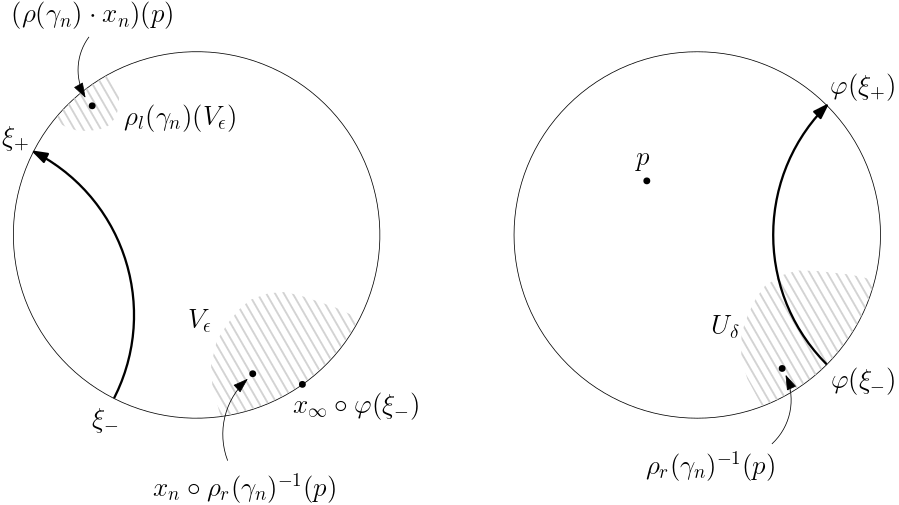
\includegraphics[width=0.7\textwidth]{dynamics.png}
    \caption{\red{mettere caption e rivedere positiong della figura}}
\end{figure}
Now we prove that the MHG constructed in Proposition \ref{prop:MGH_example} are all the MGH spacetime of genus $n$.
\begin{lemma}
    Let $\rho=(\rho_l,\rho_r)$ be a pair of positive Fuchsian representetion, and $\varphi :\S \to \S$ be the unique $(\rho_l,\rho_r)$-equivariant orientation-preserving homeomorphism of $\S$. Then $\Lambda(\rho)$ is the unique proper achronal meridian in $\partial \A^{2,1}$ invariant under the action of $\rho(\pi_1(\Sigma_n))$.
\end{lemma}
\begin{proof} 
    Let $\Lambda$ be a proper achronal meridian invariant under the action of $\rho(\pi_1(\Sigma_n))$. We claim $\Lambda \cap \Lambda(\rho)$ is not empty.\\
    Let $\gamma$ be a non-trivial element in $\pi_1(\Sigma_n)$. $\rho_l(\gamma)$ and $\rho_r(\gamma)$ are necessarely hyperbolic elements in $\PSL$, being $\Sigma_n$ compact, and we denote by $\xi^+_l(\gamma)$ and $\xi^+_r(\gamma)$ their attractive fixed points respectively. We have that $\xi^+_r(\gamma) = \varphi(\xi^+_l(\gamma))$, hence
    \[
        (\xi^+_l(\gamma), \xi^+_r(\gamma)) \in \Lambda(\rho).
    \]
    Now, the curve $\Lambda$ must meet the leaf of the left ruling of $\partial \A^{2,1}$
    \[
        \lambda_{\xi^+_r(\gamma)} = \{ (x, \xi^+_r(\gamma)) \ | \ x\in \S \}
    \]
    in a point $(x_0, \xi^+_r(\gamma))$. Then $(\rho_l(\gamma)^k \cdot x_0 ,\xi^+_r(\gamma)) \in \Lambda$ for $k>0$ and, if $x_0\neq \xi^-_l(\gamma)$, passing to the limit on $k$ we have that $(\xi^+_l(\gamma),\xi^+_r(\gamma))$ lies in $\Lambda$.\\
    To conclude assume by contradiction that for every $\gamma \in \pi_1(\Sigma_n)$ the point $(\xi^-_l(\gamma),\xi^+_r(\gamma))$ lies in $\Lambda$. Take $\alpha , \beta \in \pi_1(\Sigma_n)$ so that the axis of $\rho_l(\alpha)$ and $\rho_l(\beta)$ do not intersect. We may assume that the cyclic order of the end points of those axis is
    \begin{equation}\label{eq:order}
        \xi^+_l(\alpha) < \xi^+_l(\beta) < \xi^-_l(\beta) < \xi^-_l(\alpha).
    \end{equation}
    Since $\xi^\pm_r(\alpha) = \varphi(\xi^\pm_l(\alpha))$ and $\xi^\pm_r(\beta) = \varphi(\xi^\pm_l(\beta))$, equation \ref{eq:order} holds if we replace $\rho_l$ with $\rho_r$.
    On the other hand we assumed that $\Lambda$ contains $(\xi^+_l(\alpha), \xi^-_r(\alpha))$, $(\xi^+_l(\beta), \xi^-_r(\beta))$, $(\xi^-_l(\beta), \xi^+_r(\beta))$, $(\xi^-_l(\alpha), \xi^+_r(\alpha))$. By achronality of $\Lambda$, the cyclic order of the first and second components must be the same, hence
    \[
        \xi^-_l(\alpha) \leq \xi^-_l(\beta) \leq \xi^+_l(\beta) \leq \xi^+_l(\alpha),
    \]
    which contradicts equation \ref{eq:order}.
\end{proof}
We proved that given a pair $\rho = (\rho_l,\rho_r)$ of positive Fuchsian representations of $\pi_1(\Sigma_n)$ the MGH spacetime $M_\rho := \Omega_\rho / \rho(\pi_1(Sigma_n))$ is the unique MGH spacetime with holonomy $\rho$.\\
The last step for the classification result is that given a MGH spacetime, the left and right components of the holonomy are necessarely positive Fuchsian.

\begin{observation}\label{rem:bundle}
    By a result of Goldman \cite{goldman1980discontinuous}, a representetion $\rho$ is positive Fuchsian if and only if the associated flat $\S$ bundle $E_\rho$, constructed as the quotient of $\widetilde{\Sigma}_n \times \S$ by the diagonal action of $\pi_1(\Sigma_n)$ given by deck transformation on the first factor and by $\rho$ on the second factor, has Euler class $2-2n$. This is also equivalent to the existence of an orientation-preserving fiber bundle isomorphism between $E_\rho$ and the unit tangent bundle of $\Sigma_n$.
\end{observation}
\begin{proposition}
    Let $M$ be an oriented, time-oriented, globally hyperbolic spacetime of genus $n\geq 2$ and let us endow a Cauchy surface $\Sigma$ with the orientation induced by the future normal vector. Then the left and right components of the holonomy $\rho=(\rho_l,\rho_r): \pi_1(\Sigma)\to\PSL\times\PSL$ are positive Fuchsian representetion.
\end{proposition}
\begin{proof}
    By remark \ref{rem:bundle} we have to prove that the $\S$-flat bundles with holonomy $\rho_l$ and $\rho_r$ are isomorphic to the unit tangent bundle. We focus on $\rho_l$, the proof for $\rho_r$ is analogous.\\
    Define $\Phi_l : T^1 \widetilde{\Sigma} \to \widetilde{\Sigma} \times \S$ in the following way: for an element $(x,v) \in T^1 \widetilde{\Sigma}$ let
    \[
        \xi(x,v) = (\xi^l(x,v), \xi^r(x,v)) \in \T
    \]
    be the end-point of the spacelike geodesic ray $exp_x(tv)$ in $\A^{2,1}$, for positive $t$. We define $\Phi_l(x,v)=(x, \xi^l(x,v))$. This map is clearly continuous, proper,
    equivariant and fiber preserving.\\
    To prove that it is bijective it is sufficient to notice that for any $x \in \widetilde{\Sigma}$ the map $\xi_x : T^1_x \widetilde{\Sigma} \to \T$ is an embedding with image the boundary of the totally geodesic plane tangent to $\widetilde{\Sigma}$ at $x$. This boundary is the graph of an orientation-preserving map of $\S$, so the projection $v \to \xi^l(x,v)$ is bijective. Moreover, by the choice of the orientation on $\Sigma$, the orientation on $T^1_x \widetilde{\Sigma}$ corresponds to the orientation induced on $\xi_x (T^1_x \widetilde{\Sigma})$ as graph of an orientation-preserving homeomorphism.
\end{proof}

We conclude this section by stating the classification result. Let the \emph{deformation space} of MGH spacetimes of genus $n$ be:
$$\mathcal{MGH}(\Sigma_n)=\{g\text{ MGH AdS metric on }\Sigma_r\times\R\}/\mathrm{Diff}_0(\Sigma_n\times\R)~,$$
where the group of diffeomorphisms isotopic to the identity acts by pull-back. The holonomy map takes value in the space of representations of $\pi_1(\Sigma_r)$ into $\PSL\times\PSL$ and is well-defined on the quotient $\mathcal{MGH}(\Sigma_r)$.
We proved that the left and right components of the holonomy of elements of $\mathcal{MGH}(\Sigma_n)$ are positive Fuchsian representations, and the space of these representations up to conjugacy is identified with the Teichm\"uller space of $\Sigma_n$
\[
    \mathcal{T}(\Sigma_n)\cong\{\rho:\pi_1(\Sigma_n)\to\PSL\text{ positive Fuchsian representations}\}/\PSL~.
\]
Therefore the holonomy map can be considered as a map 
from $\mathcal{MGH}(\Sigma_n)$ with values in $\mathcal{T}(\Sigma_n)\times\mathcal{T}(\Sigma_n)$.
Hence, we can summarize this section with the following theorem of Mess.

\begin{theorem} \label{thm:classification rgeq2}
The holonomy map $$\rho:\mathcal{MGH}(\Sigma_n)\to\mathcal{T}(\Sigma_n)\times\mathcal{T}(\Sigma_n)$$ is a homeomorphism.
\end{theorem}